\documentclass{article}
\usepackage[utf8]{inputenc}
\usepackage{graphicx}
\usepackage{subcaption}
 
\graphicspath{{Images/}}
\title{Thesis}
\author{John DeCorato}
\date{ }
 
\begin{document}
 
\maketitle
 
\tableofcontents
 
\section{Introduction}

\section{Related Work}

\subsection{2-D Drawing}

Illustrator http://www.adobe.com/products/illustrator.html

Illustrator is a vector graphics editor made by Adobe Software. It uses geometric primitives such as points, lines, curves, and polygons to create images. The current version, Illustrator CC, is the seventeenth edition of the product.

Sketchbook Pro http://www.autodesk.com/products/sketchbook-pro/features/all/gallery-view

Mischief https://www.madewithmischief.com/

Mischief is another vector graphics editor created by Made With Mischief, now owned by The Foundry. It features an infinite canvas for a free-form and dynamic sketching environment. This is allowed by using a data-structure called Adaptive Distance Fields, which allows them to greatly reduce the storage size of the vectors that the user creates at the cost of the ability to edit the vectors. 


\subsection{3-D Modeling in CAD}

Rhino

AutoCAD

Maya / 3DMAX

Sketchup

\subsection{3-D Sketching in CAD}

\subsubsection{CATIA Natural Sketch}

\begin{figure}[h!]

\begin{subfigure}{\textwidth}
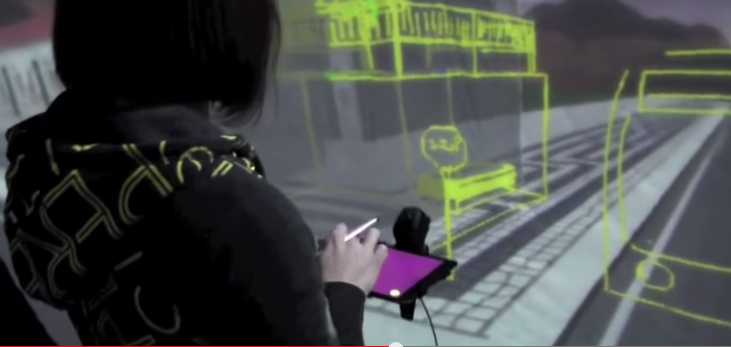
\includegraphics[width=0.9\linewidth]{Hyve3D1}
\caption{Using the tablet to draw}
\end{subfigure}
\begin{subfigure}{\textwidth}
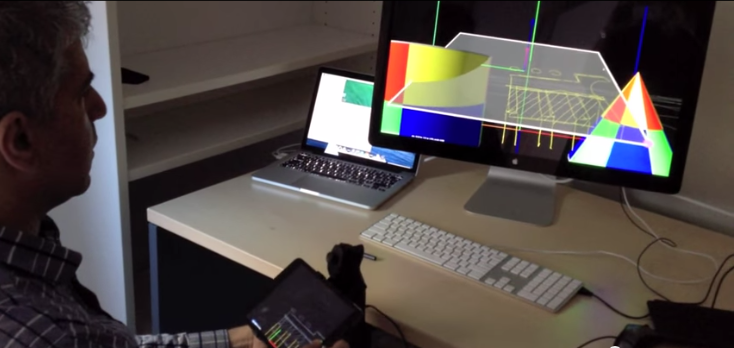
\includegraphics[width=0.9\linewidth]{Hyve3D2}
\caption{Manipulating the drawing plane}
\end{subfigure}

\caption{Examples of Hyve 3-D in use}
\end{figure}

Natural Sketch is a feature inside of the CATIA modeling software by Dassault Systemes. Natural Sketch allows the user to draw on a virtual plane, a 3-D model, and the plane where the screen lies in the 3D environment. It features the abilities to alter the pen style, alter the number of control points used to make the post sketch curve, automatically change the camera view to align with the drawing plane if one is being used, copy and alter individual strokes, and generate models from the 3-D sketch.




\subsubsection{ILoveSketch / EverybodyLovesSketch}

EverybodyLovesSketch is a 3D curve sketching system from the University of Toronto's Dynamic Graphics Project Lab. It features a pen based gesture system, allowing the user to execute functions using rapid strokes, circles, and other defined gestures. Other features include dynamic sketch plane selection, single view definition of arbitrary extrusion vectors, multiple extruded surface sketching, copy-and-project of 3D curves, free-form surface sketching, and an interactive perspective grid. This project is based off of previous work by the same lab, ILoveSketch, which is the base 3D sketching functionality of the EverybodyLovesSketch project.

\subsubsection{Hyve 3D}

\begin{figure}[h]

\begin{subfigure}{\textwidth}
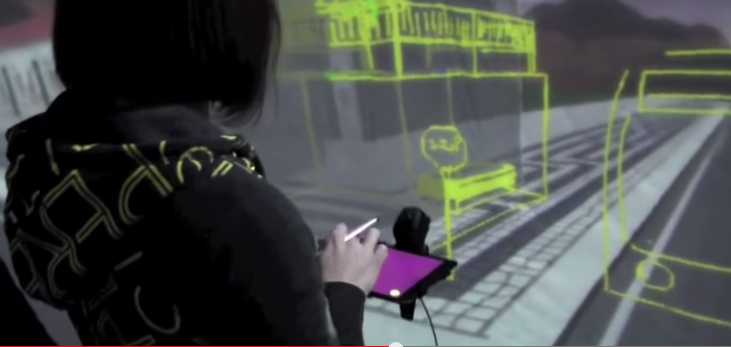
\includegraphics[width=0.9\linewidth]{Hyve3D1}
\caption{Using the tablet to draw}
\end{subfigure}
\begin{subfigure}{\textwidth}
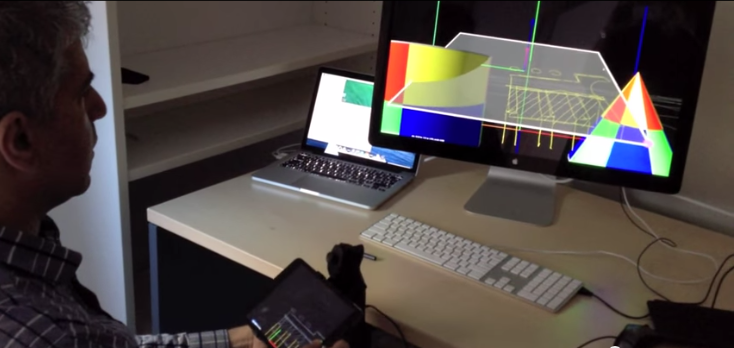
\includegraphics[width=0.9\linewidth]{Hyve3D2}
\caption{Manipulating the drawing plane}
\end{subfigure}

\caption{Examples of Hyve 3-D in use}
\end{figure}

Hyve 3D is an infinite virtual sketching environment from the University of Montreal. It uses two screens; a computer monitor to show the 3-D environment, and an iPad to draw. The sketching plane represented by the iPad is shown in the virtual environment, and is manipulated by moving and rotating the iPad in the real world. The user then pins the sketch plane in place and proceeds to draw at leisure.



\subsection{Other Work in 3-D Sketching}

Augmented Reality In-Situ 3D Sketching of Physical Objects $http://creativemachines.cornell.edu/papers/IUI09_Yee.pdf$

Gravity http://gravitysketch.com/

Gravity is an augmented reality 3D sketching tool using a tablet as the sketch base and a wearable screen to show the sketch. The tablet acts as a drawing plane, while the sketch can be moved via a set of controls on the tablet. The main idea is similar to Hyve 3D, in that you always draw in 2-D while you use your own sense of depth and position to understand what you are drawing, allowing for 3-D sketching without the use of perspective drawing. The difference is that this system allows you to use real world depth cues to augment your understanding of the virtual 3-D environment.

Sketch http://graphics.cs.brown.edu/research/sketch/

Polyes Q1 Pen http://technabob.com/blog/2014/12/29/polyes-q1-3d-sketching-pen/

\subsection{3-D Media Interaction}

Gestures vs. Postures: ‘Gestural’ Touch Interaction in 3D Environments 

\begin{verbatim}
$http://tobias.isenberg.cc/personal/papers/Isenberg_2012_GPG.pdf$
\end{verbatim}
A Survey of Interaction Techniques for Interactive 3D Environments http://www.grey-eminence.org/papers/EG2013-STAR.pdf

Interaction with 3-D environments using Multitouch Screens $http://www.researchgate.net/publication/236304194_Interaction_with_3D_Environments_using_Multi-Touch_Screens$

\subsection{Touch Based User Interfaces}

Dual touch: a two-handed interface for pen-based PDAs
\begin{verbatim}
$http://vp5qw4uf5x.scholar.serialssolutions.com/?sid=google&auinit=N&aulast=Matsushita&atitle=Dual+touch:+a+two-handed+interface+for+pen-based+PDAs&id=doi:10.1145/354401.354774$
\end{verbatim}
\subsection{Pen Based User Interfaces}

Pen Based Interaction 
\begin{verbatim}
$http://www.academia.edu/2236260/Pen-based_Interaction_-_Next_Generation_User_Interfaces_WE-DINF-15756_$
\end{verbatim}
Pen-based User Interface 
\begin{verbatim}
$http://ieeexplore.ieee.org/stamp/stamp.jsp?tp=&arnumber=1349146$
\end{verbatim}
Experimental Analysis of Mode Switching Techniques in Pen-based User Interfaces http://research.microsoft.com/en-us/um/people/kenh/papers/p226-li.pdf

\section{The Design Process}

\subsection{Conceptual Design}

\subsection{Computer Aided Design}

\subsection{Computer Aided, Early Phase Design}

\section{Input}

\subsection{Pen}

\subsection{Touch}

\subsection{Gesture}

\section{Splines}

Curve Global Interpolation http://www.cs.mtu.edu/~shene/COURSES/cs3621/NOTES/INT-APP/CURVE-INT-global.html

Smooth Spline Through Prescribed Points https://www.particleincell.com/2012/bezier-splines/

\subsection{Definition of Splines}

\subsection{Construction}

\subsection{Inverse Spline Calculation}

\section{Sketching in 3-D}

\subsection{Ray Casting}

\subsection{User Input}

\section{Usability and Feel: Bringing Physical Tools to the Virtual World}

\subsection{Interacting with the 3D environment}

\subsection{Connecting 2-D and 3-D}

\subsection{Combining Pen and Touch}

\subsection{Recreating the Feel of the Real World}
 
\end{document}